% !TeX root = RJwrapper.tex
\title{Seasonal Adjustment of Daily Time Series in R: An Overview}
\author{by Christoph Sax, Author Two, and Author Three}

\maketitle

\abstract{%
This {[}article/chapter/post{]} discusses available methods for high
frequency seasonal adjustment in R. It focuses on the adjustment of
daily data, but also includes examples of weekly data. We discuss the
literature and provide an overview of the available methods, including
user examples. The methods are evaluated in two different ways: First we
perform an out-of-sample forecast evaluation. Second, we compare the
adjusted series with the results of X13, an established method for
seasonal adjustment of monthly data. Finally, we discuss some specific
problems of seasonal adjustment.
}

\hypertarget{introduction}{%
\subsection{Introduction}\label{introduction}}

Automated data processing and the Internet have brought an enormous
increase in data that is processed on a high frequency, e.g., at a
daily, hourly or even higher frequency. While some higher frequency
series have been used in the past (e.g., Fisher 1923, cited by Ladiray
2018) these series are much more abundant now. X-13ARIMA-SEATS offers a
well-tested and time proven way of adjusting monthly, quarterly (or
bi-annual) series, but it cannot deal with data at a higher frequency.

This {[}article/chapter/post{]} discusses how to perform seasonal
adjustment on a higher frequency. We focus on daily data, as this is the
most common use case, but will briefly discuss some challenges involving
weekly or intra-day adjustments.

Despite the large interest, there is not much consensus on the
appropriate adjustment method for daily series. Adjusting daily series
often involves a substantial amount of trial and error, subjective
judgment and exploration. This {[}article/chapter/post{]} gives an
overview of the tools that are currently (2021) available in R.

The focus is both on the usage and on the methodology. We try to give
usage example for each method and try to cover them in a unified manner.

We first give a short methodologial overview ob daily seasonal
adjustment and disuss some specifi problems that come with high
frequency seasonal adjustment. We then discuss various R packages that
can be used to perform high frequency seasonal adjustment. In the
`Evaluation' chapter, we compare the results of these packages, and give
some advice on the selction of an optimal method. Further topics of high
frequency seasonal adjustment are discussed in the final chapter.

\hypertarget{overview}{%
\subsection{Overview}\label{overview}}

\hypertarget{problems-of-high-frequency-adjustments}{%
\subsection{Problems of High Frequency
Adjustments}\label{problems-of-high-frequency-adjustments}}

Daily seasonal adjustment comes with a few challenges that are not
present in lower frequency data. Let's focus on daily traffic
casualties.

First, daily data comes at multiple periodicities: There is an annual
periodicity, such as the effect of weather conditions or holiday
patterns. Then there is a weekly periodicity. Casualties may be higher
during the weekdays, due to increased work traffic. For some series,
there may be also a monthly periodicity. If people get their salaries by
the end of the month, they may be more likely to perform certain
investments.

Second, many daily data series are available for a few years only.
Whily, e.g., the SEATS adjustment requires a minimal series length of XX
years, many daily series are shorter.

Third, higher frequency series are generally more volatile and prone to
outliers.

Fourth, the effect of individual holiday is challenging to estimate.
Often, economic effects of holidays may occur before or after a holiday,
thus lagging or leading them is crucial.

\hypertarget{parametric-versus-non-parametric-models}{%
\subsection{Parametric versus Non-parametric
Models}\label{parametric-versus-non-parametric-models}}

Various attempts to seasonly adjust data can be broadly distinguished
into parametric and non-parametric approaches. Non-parametric approaches
seem to be the more obvious candidates to use with the irregular
structure of daily data. Parametric models require the time units to be
regularly spaced. Non-parametric estimation is also what is used in the
X-11 method of X-13.

\hypertarget{r-packages}{%
\subsection{R Packages}\label{r-packages}}

As mentioned before, there is no accepted consensus on how to perform
daily seasonal adjustment. In the following, we discuss various
possibilities to adjust series in R. We focus on a single time series,
and describe the concrete steps that are required to perform an
adjustment.

\emph{dailyadj} is an R package to accompany this article. It can can be
donloaded from GitHub {[}needs to be published.{]}. It contains various
daily example series. In the following, we focus on UK traffik
casualities from 2005 to 2016.

\begin{Schunk}
\begin{Sinput}
library(dailyadj)
library(tsbox)
library(tidyverse)

casualties
\end{Sinput}
\begin{Soutput}
#> # A tibble: 4,383 x 2
#>    time       value
#>    <date>     <dbl>
#>  1 2005-01-01   452
#>  2 2005-01-02   468
#>  3 2005-01-03   418
#>  4 2005-01-04   599
#>  5 2005-01-05   686
#>  6 2005-01-06   710
#>  7 2005-01-07   656
#>  8 2005-01-08   601
#>  9 2005-01-09   520
#> 10 2005-01-10   688
#> # ... with 4,373 more rows
\end{Soutput}
\end{Schunk}

We store high frequency time series in an R data frame, specifically in
a \emph{tibble}. This data frame has a \texttt{time} and a
\texttt{value} column. This has two major advantages to other classes,
such as \texttt{ts}. First, it does not force the data into any kind of
regularity. February 29 data, if it orrucs, can be stored without
problems. Second, R has offers a pleotora of tools to perform fantastic
stuff with data frames, while we have less tools available for other
classes. Here, and throughtout the article, we use \emph{tsbox} and
\emph{tidyverse} to simplify the data manipulation. \texttt{ts\_plot()}
offers a convenient way to plot this tabular data (or any other time
series data):

\begin{Schunk}
\begin{Sinput}
ts_plot(casualties)
\end{Sinput}

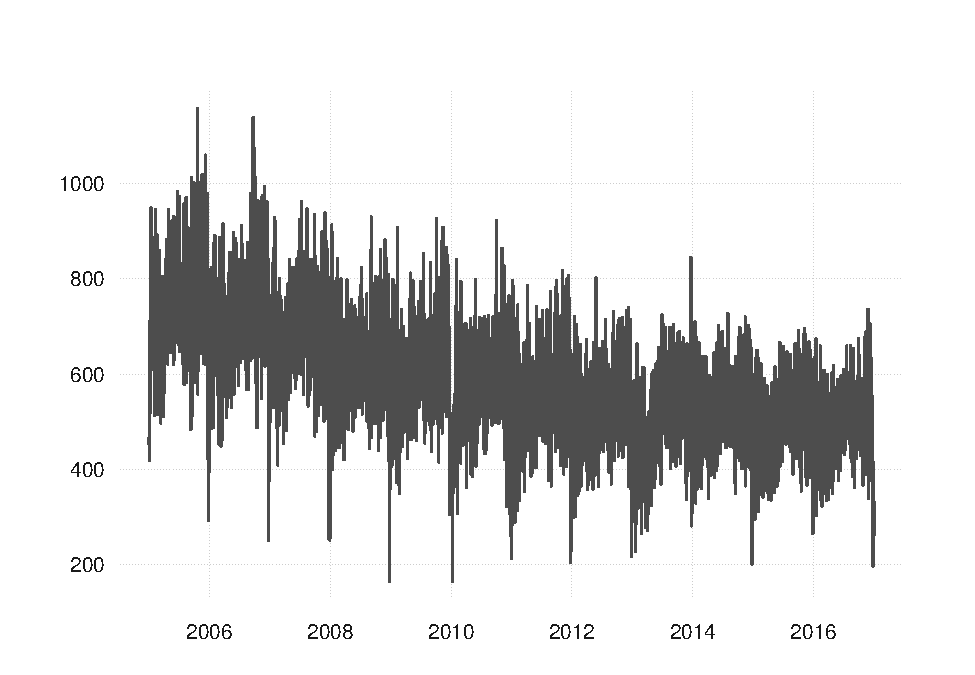
\includegraphics[width=1\linewidth]{overview_files/figure-latex/unnamed-chunk-2-1} \end{Schunk}

\hypertarget{arima-month-weekday-holiday-dummies}{%
\subsection{ARIMA + Month, Weekday / Holiday
Dummies}\label{arima-month-weekday-holiday-dummies}}

Perhaps the simplest way to seasonally adjust a high frequency time
series is to use dummies to control for month or weekday effects. As we
will see, these models have some considerable drawbacks, but their
discussing may be helpful nevertheless. Also, these kinds of adjustments
are frequently found in the literature. E.g., timmermans 18,
\href{https://sjes.springeropen.com/articles/10.1186/s41937-020-00052-y}{lengwiler
20}.

We start by constructing a dummy variable with weekday and monthly
effects:

\begin{Schunk}
\begin{Sinput}
dums <-
  casualties %>%
  mutate(wday = lubridate::wday(time, label = TRUE)) %>%
  mutate(month = lubridate::month(time, label = TRUE)) %>%
  select(time, wday, month) %>%
  fastDummies::dummy_cols("wday", remove_selected_columns = TRUE) %>%
  fastDummies::dummy_cols("month", remove_selected_columns = TRUE) %>%
  select(-wday_Mon, -month_Jan)

dums
\end{Sinput}
\begin{Soutput}
#> # A tibble: 4,383 x 18
#>    time       wday_Sun wday_Tue wday_Wed wday_Thu wday_Fri wday_Sat month_Feb
#>    <date>        <int>    <int>    <int>    <int>    <int>    <int>     <int>
#>  1 2005-01-01        0        0        0        0        0        1         0
#>  2 2005-01-02        1        0        0        0        0        0         0
#>  3 2005-01-03        0        0        0        0        0        0         0
#>  4 2005-01-04        0        1        0        0        0        0         0
#>  5 2005-01-05        0        0        1        0        0        0         0
#>  6 2005-01-06        0        0        0        1        0        0         0
#>  7 2005-01-07        0        0        0        0        1        0         0
#>  8 2005-01-08        0        0        0        0        0        1         0
#>  9 2005-01-09        1        0        0        0        0        0         0
#> 10 2005-01-10        0        0        0        0        0        0         0
#> # ... with 4,373 more rows, and 10 more variables: month_Mar <int>,
#> #   month_Apr <int>, month_May <int>, month_Jun <int>, month_Jul <int>,
#> #   month_Aug <int>, month_Sep <int>, month_Oct <int>, month_Nov <int>,
#> #   month_Dec <int>
\end{Soutput}
\end{Schunk}

These variables can be used as exogenous variables in a ARIMA model. We
use \texttt{forecast::auto.arima()} to determine the ARMA order. Note
that we do not want to use the seasonal part of the model, since we use
dummies for this purpose.

\begin{Schunk}
\begin{Sinput}
fit <- auto.arima(casualties$value, seasonal = FALSE, xreg = as.matrix(dums[, -1]))
adj <- casualties
adj$value <- as.numeric(fit$fitted)

ts_plot(casualties, adj)
\end{Sinput}

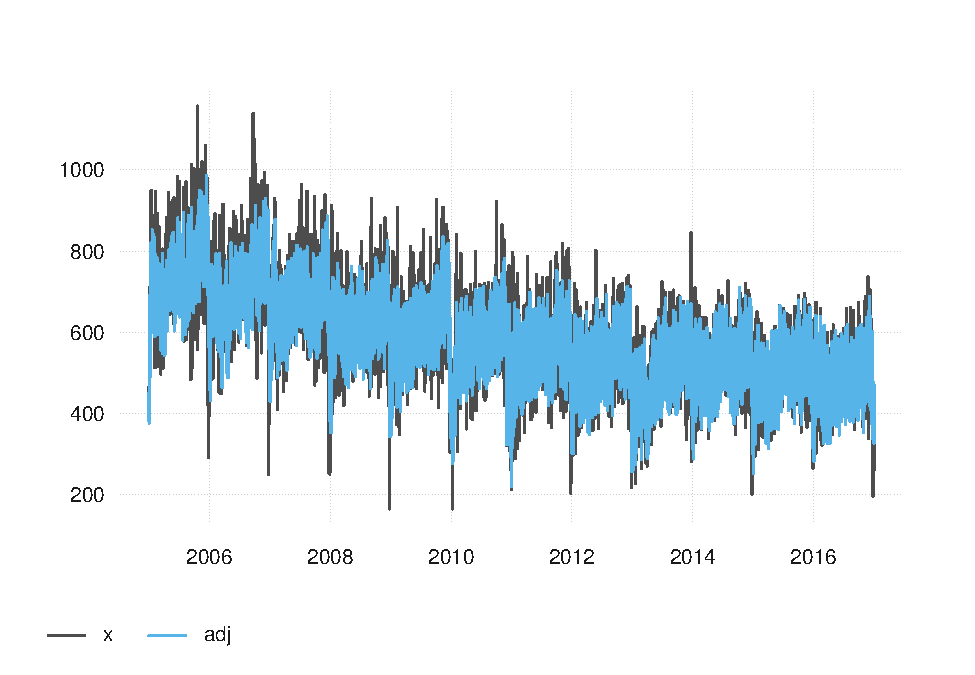
\includegraphics[width=1\linewidth]{overview_files/figure-latex/arimax-1} \end{Schunk}

The nice think about the dummy model is that its seasonal effects are
very easy to interprete. By construction, they are constant over time,
and can be visualized as follows:

\begin{Schunk}
\begin{Sinput}
enframe(coef(fit)) %>%
  filter(grepl("wday", name)) %>%
  mutate(name = gsub("wday_", "", name)) %>%
  mutate(name = factor(name, levels = unique(name))) %>%
  ggplot(aes(x = name, y = value)) +
    geom_col() +
    ggtitle("Weekday effects", subtitle = "Baseline: Monday")
\end{Sinput}

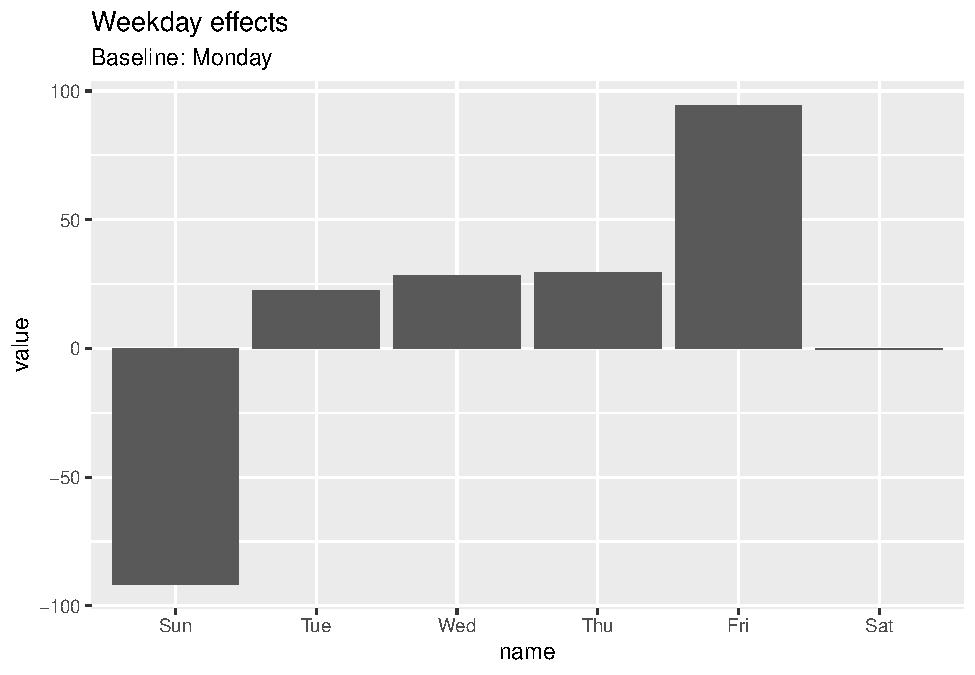
\includegraphics[width=1\linewidth]{overview_files/figure-latex/coeff-plots-1} \begin{Sinput}
enframe(coef(fit)) %>%
  filter(grepl("month", name)) %>%
  mutate(name = gsub("month_", "", name)) %>%
  mutate(name = factor(name, levels = unique(name))) %>%
  ggplot(aes(x = name, y = value)) +
    geom_col() +
    ggtitle("Month effects", subtitle = "Baseline: January")
\end{Sinput}

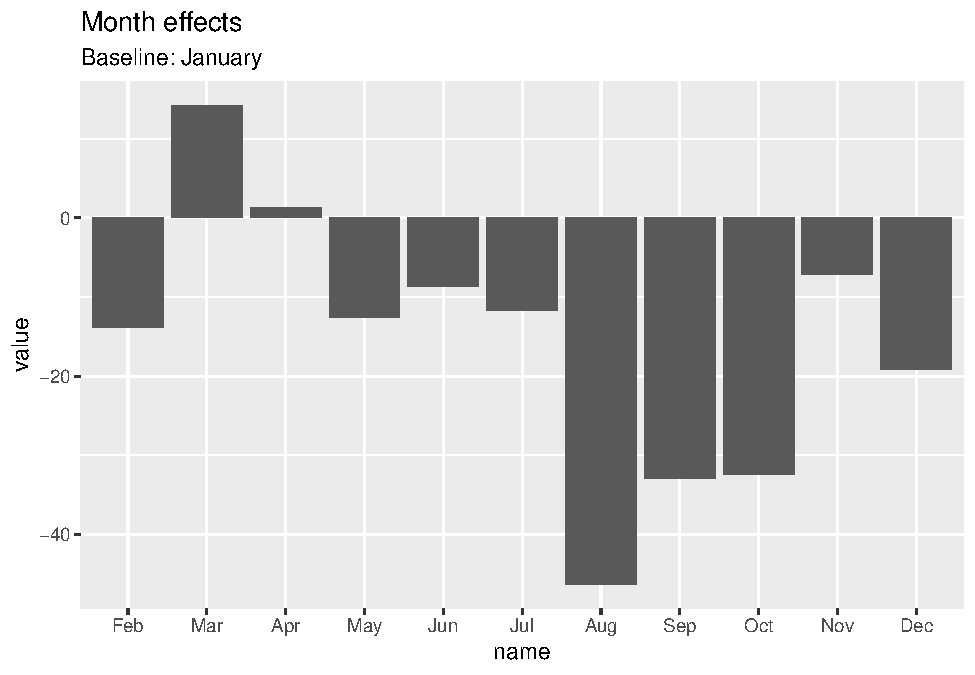
\includegraphics[width=1\linewidth]{overview_files/figure-latex/coeff-plots-2} \end{Schunk}

We see that, on average, traffic casualties are lower on Sunday and peak
on Friday. We also see that, on average, casualties are sligthly lower
in early autumn.

\hypertarget{stl}{%
\subsection{STL}\label{stl}}

While dummy models are easy to estimate and iterprete, they have a
substantial drawback: Their effects are typically \emph{time-invariant},
which is rarely a good assumption. Where we look at weekday or month
effects, these effects are likely to change over time.

A straigthforward solution is to estimate these effects
non-parametrically. Fundamentally, this uses the same idea as the
ubiquitous X-11 method, wich is used by X13, the seasonal adjustment
method by the US Census bureau.

STL (Cleveland et al, 1990, seasonal-trend decomposition procedure based
on loess) follows a similar idea but uses local regressions to estimate
seasonal effects that may change over time. R base has a function
\texttt{stl()} that performs this decompostion, but it requires the data
to be equispaced. Models with an equispace requirement will be discusses
later on.

However, STL can be applied to irregular data as well. The basic idea is
to align all weekdays and draw a smoothed line through these data
points. This is you initial estimation of a \emph{weekday} effect, which
will be substracted from a detrended series. Secondly, the days of a
month or a year may be aligned, leading an estimation of a monthly or
yearly effect. Once all effects are estimated, the procedure may be
repeated, with an iteratively improved trend estimation.

\emph{dailyseas} contains a simple implementation of STL that works in
many circumstances. See the source code of \texttt{seas\_daily()}, which
uses relatively simple dplyr manipulations.

\begin{Schunk}
\begin{Sinput}
casualties %>%
  seas_daily() %>%
  ts_pick("orig", "adj") %>%
  ts_plot()
\end{Sinput}

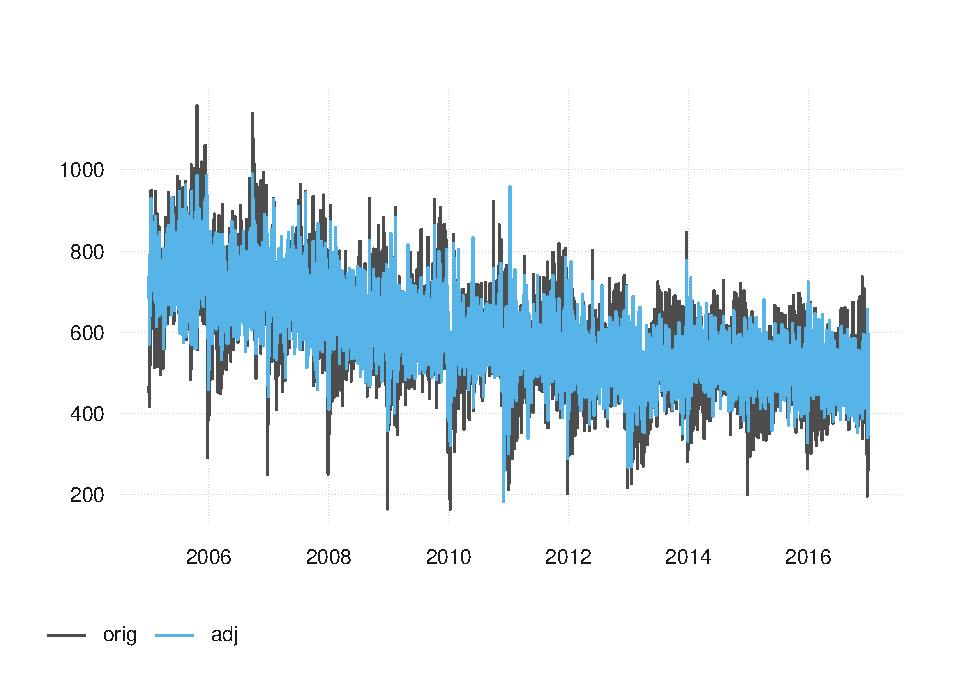
\includegraphics[width=1\linewidth]{overview_files/figure-latex/stl-1} \end{Schunk}

\hypertarget{dsa}{%
\subsection{dsa}\label{dsa}}

In a very similar spirit, the dsa packages implements a version of STL.
It is computationally much more intensive, as it performs extensive
outlier adjustments.

The following code autmatically decomposes \texttt{casulties}, using the
\emph{dsa} package:

\begin{Schunk}
\begin{Sinput}
library(dsa)
z <- dsa::dsa(ts_xts(casualties))
\end{Sinput}
\begin{Soutput}
#>   |                                                                              |                                                                      |   0%  |                                                                              |===                                                                   |   5%  |                                                                              |=======                                                               |  10%  |                                                                              |====================                                                  |  29%  |                                                                              |===========================                                           |  38%  |                                                                              |===============================================                       |  67%  |                                                                              |==================================================                    |  71%  |                                                                              |=====================================================                 |  76%  |                                                                              |===============================================================       |  90%  |                                                                              |======================================================================| 100%
\end{Soutput}
\begin{Sinput}
plot(z, dy = FALSE)
\end{Sinput}

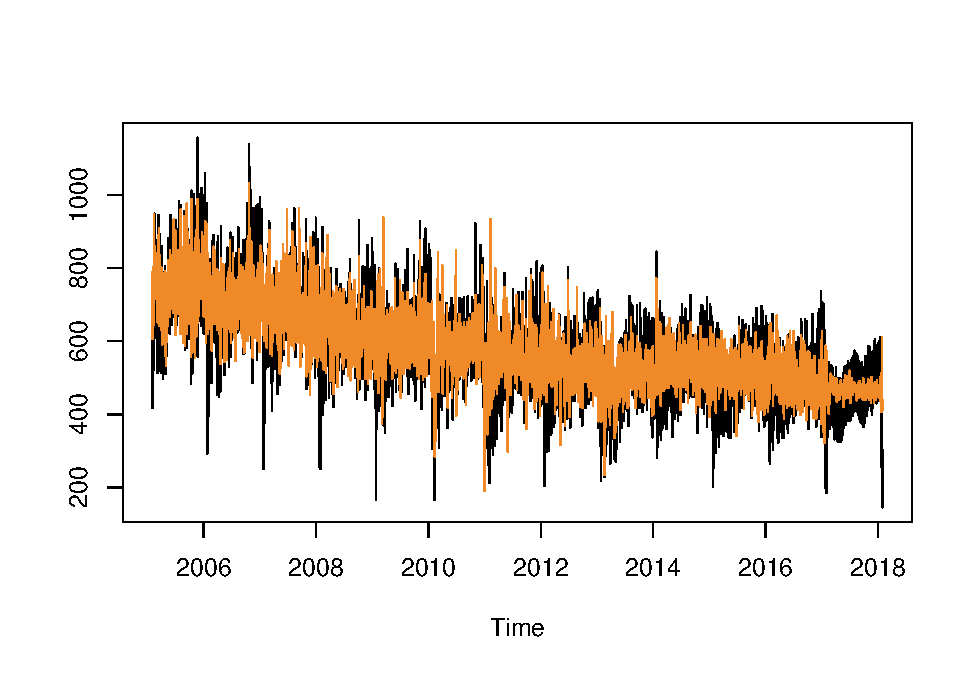
\includegraphics[width=1\linewidth]{overview_files/figure-latex/dsa-1} \end{Schunk}

\hypertarget{prophet}{%
\subsection{prophet}\label{prophet}}

The \emph{prophet} packages promises an automated approach to
forecasting and decomposing high frequency time series. Like the
procedures above, it does not require the data to be equispaced. (Taylor
SJ, Letham B. 2017)

At its core, the Prophet procedure is an additive regression model with
four main components:

A trend, a yearly seasonal component, a weekly weekly seasonal component
and a user-provided list of important holidays. This is fundamentally no
different to the STL methods above. However, for trend estimation,
prophet uses a piecewise linear or logistic growth curve trend, for
yearl effect, is ueses Fourier series. As the dummy model in the
beginning, it uses dummy variables to estimate the trend.

In order to prepare the data, column names need be changed to
\emph{prophet}'s defaults. Estimation is specified using
\texttt{prophet()}. Country specific holiday effects can be added.
Acutal fitting is done by \texttt{fit.prophet()}:

\begin{Schunk}
\begin{Sinput}
library(prophet)

df <- rename(casualties, ds = time, y = value)
m <-
  prophet(daily.seasonality = FALSE) %>%
  add_country_holidays(country_name = 'UK') %>%
  fit.prophet(df)
\end{Sinput}
\end{Schunk}

The seasonally decomposed series (and a forecast) can be extracted as
follows:

\begin{Schunk}
\begin{Sinput}
# not strictly needed, but will include forecast too
future <- make_future_dataframe(m, periods = 31)
forecast <- as_tibble(predict(m, future))

forecast %>%
  transmute(
    time = as.Date(ds),
    additive_terms,
    yhat
  ) %>%
  left_join(casualties, by = "time") %>%
  mutate(adj = value - additive_terms) %>%
  select(time, value, adj) %>%
  ts_long() %>%
  ts_plot()
\end{Sinput}

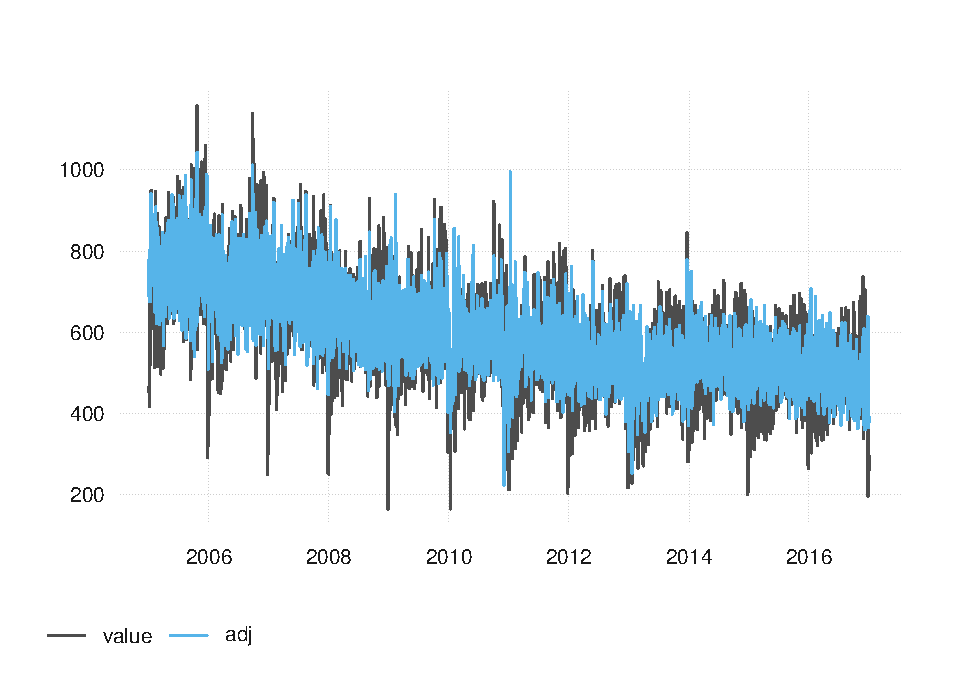
\includegraphics[width=1\linewidth]{overview_files/figure-latex/prophet-components-1} \end{Schunk}

\hypertarget{tbats}{%
\subsection{TBATS}\label{tbats}}

The previous models did not require the data to be equispaced. However,
modelling techniques have been developed in the context of monthly or
quarterly data. They often assume that each low frequency period must
include the exact same number of high frequency periods.

With daily data (or much worse, weekly data, which will be discussed
below), this is not the case. A year may have 365 or 366 days, and it is
not always clear how the February 29 problem should be handled.

\texttt{ts\_ts} from the tsbox package offers an easy way to convert
daily data into regular \texttt{"ts"} objects with a frequency of
365.2425. Thus, days are slightly offset in each year.

\begin{Schunk}
\begin{Sinput}
x_ts <- ts_ts(casualties)
head(x_ts)
\end{Sinput}
\begin{Soutput}
#> Time Series:
#> Start = 2005 
#> End = 2005.01368953503 
#> Frequency = 365.2425 
#> [1] 452 468 418 599 686 710
\end{Soutput}
\end{Schunk}

TBATS Models (De Livera, Hyndman, \& Snyder, 2011) require the data to
be equispaced.

\begin{Schunk}
\begin{Sinput}
fit <- tbats(x_ts)
adj <- fit$fitted
ts_plot(casualties, adj)
\end{Sinput}

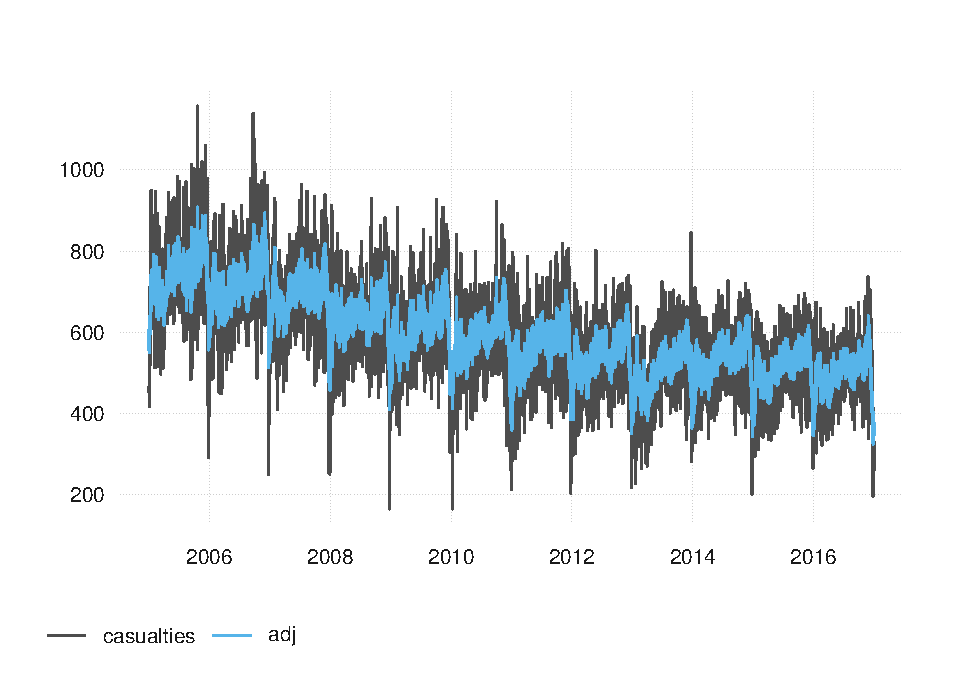
\includegraphics[width=1\linewidth]{overview_files/figure-latex/tbats-1} \end{Schunk}

\hypertarget{evaluation}{%
\subsection{Evaluation}\label{evaluation}}

Which method should you choose? Various criterions could be applied. A
seasonal decomposition model can be used to perform forecasts as well.
The forecasting capability can be used for a pseudo out-of-sampe
forcasting exercise. For all the methods discussed and for a number of
time series, we perform such an exercise.

Also, a seasonally adjusted series can be compared ot established
methods of seasonal adjustment for monthly and quarterly data. In a
second excercise, we compare monthly values of adjusted series to
adjustments of X-13, using the X-11 method.

\hypertarget{out-of-sample-forecast}{%
\subsection{Out-of-sample forecast}\label{out-of-sample-forecast}}

As in (Timmermans 18), the following produces OOS forecasts for the
twelve last months for UK traffic deaths. We apply
\texttt{dailyseas::eval\_oos()} to perform an OOS forecast evaluation
for all models.

The full OOS results can be found
\href{https://github.com/christophsax/x13book/blob/master/topics/dailyadj/vignettes/overview.md}{here}

{[}I think the detailed OOS results are quite interesting, as they show
you what a method `gets' and what it does not.{]}

Here is the table for two series, showing the mean percentage deviation:

\begin{Schunk}

\begin{tabular}{lrrrr}
\toprule
model & casualties & nzimmigration\_dep & transact & nzimmigration\_arr\\
\midrule
dummy & 0.16 & 0.16 & 0.16 & 0.21\\
daily & 0.11 & 0.19 & 0.11 & 0.18\\
dsa & 0.10 & 0.12 & 0.10 & 0.16\\
prophet & 0.10 & 0.13 & 0.12 & 0.14\\
harmon & 0.12 & 0.16 & 0.15 & 0.21\\
tbats & 0.13 & 0.22 & 0.13 & 0.28\\
naive & 0.14 & 0.19 & 0.17 & 0.18\\
\bottomrule
\end{tabular}

\end{Schunk}

\hypertarget{comparison-to-x-13}{%
\subsection{Comparison to X-13}\label{comparison-to-x-13}}

For the methods and series above, we:

\begin{itemize}
\tightlist
\item
  compute adjusted series
\item
  aggregate them to monthly
\item
  compare them X13 Series
\item
  compute mpce between the two and tabluate
\end{itemize}

{[}perhaps also look at \texttt{qs()}?{]}

there is a literature on this (montly GDP vs quarterly). If a monthly
adjustment seems good but produces a bad quarterly adjustemnt, it is
probably not a good adjustment. {[}James, perhaps elaborate?{]}

\hypertarget{computation-time}{%
\subsection{Computation time}\label{computation-time}}

Finally, for practial purposes, speed may be an important consideration,
too. Differences in computational speed between the methods are large,
ranging from less than a second to serveral minutes.

\begin{verbatim}
stl (my one): 0.639
seas_dummy:   2.319
prophet:     10.181
dsa:        145.553
\end{verbatim}

\hypertarget{conclusions}{%
\subsection{Conclusions}\label{conclusions}}

\emph{prophet}, \emph{dsa}, and the simple stl procedure all work
relatively well. Working with equispaced data is much harder.

{[}Is this because I don't use the correctly? Should I just remove
Feb.~29? Grateful for a TBATS example that produces something
meaningful{]}

\hypertarget{other-challenges}{%
\section{Other challenges}\label{other-challenges}}

{[}Discuss some other challenges of daily seas adj{]}

\hypertarget{short-series}{%
\subsection{Short series}\label{short-series}}

Many daily time series are short. What does it mean with respect to the
discussion above. If I have only 3 years of data, which methods still
work?

\hypertarget{calendar-effects}{%
\subsection{Calendar effects}\label{calendar-effects}}

{[}Will try to improve my method on that, prophet and dsa do something
about it. Could provide an example, OOS comparison{]}

\hypertarget{cross-seasonal-effects}{%
\subsection{Cross Seasonal Effects}\label{cross-seasonal-effects}}

If month effects (e.g., salary payment at the end of a month) collide
with week effects (e.g., weekend), we can get some patterns that are
very hard to model. How relevant is the problem? What should you be done
about it?

\hypertarget{series-specific-effects}{%
\subsection{Series specific effects}\label{series-specific-effects}}

Transaction series have an end of months effect (Timmermans 18), but we
don't find it in other data. How to deal with such things?

\hypertarget{weekly-seasonality}{%
\subsection{Weekly seasonality}\label{weekly-seasonality}}

One solution would be to disaggregate, perform daily seasonal adjustment
and aggregate again. Could provide an example.

Compare to weekly methods?

\hypertarget{conclusions-1}{%
\section{Conclusions}\label{conclusions-1}}

\hypertarget{literature}{%
\section{Literature}\label{literature}}

Cleveland, R. B., Cleveland, W. S., McRae, J. E., \& Terpenning, I. J.
(1990). STL: A seasonal-trend decomposition procedure based on loess.
Journal of Official Statistics, 6(1), 3--33.

Lengwiler, Y. Blacking out. Swiss J Economics Statistics 156, 7 (2020).
\url{https://doi.org/10.1186/s41937-020-00052-y}

Taylor SJ, Letham B. 2017. Forecasting at scale. PeerJ Preprints
5:e3190v2 \url{https://doi.org/10.7287/peerj.preprints.3190v2}

De Livera, A. M., Hyndman, R. J., \& Snyder, R. D. (2011). Forecasting
time series with complex seasonal patterns using exponential smoothing.
J American Statistical Association, 106(496), 1513--1527.
\url{https://robjhyndman.com/publications/complex-seasonality/}

Timmermans, Monique, Ronald Heijmans, and Hennie Daniels. ``Cyclical
patterns in risk indicators based on financial market infrastructure
transaction data.'' (2017).

\hypertarget{appendix}{%
\section{Appendix}\label{appendix}}

\hypertarget{components-plots}{%
\subsubsection{Components Plots}\label{components-plots}}

\hypertarget{casualties-prophet}{%
\paragraph{Casualties, Prophet}\label{casualties-prophet}}

\begin{Schunk}
\begin{Soutput}
#> Warning: Removed 31 row(s) containing missing values (geom_path).
\end{Soutput}

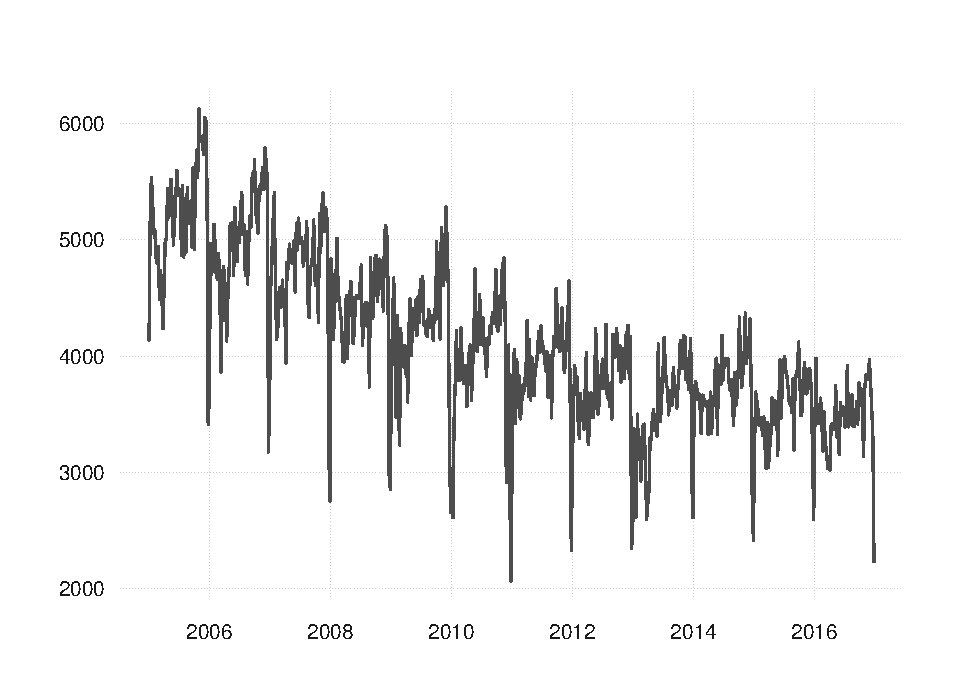
\includegraphics[width=1\linewidth]{overview_files/figure-latex/unnamed-chunk-5-1} \end{Schunk}

\hypertarget{casualties-dsa}{%
\paragraph{Casualties, DSA}\label{casualties-dsa}}

\begin{Schunk}
\begin{Soutput}
#> Warning: Removed 40 row(s) containing missing values (geom_path).
\end{Soutput}

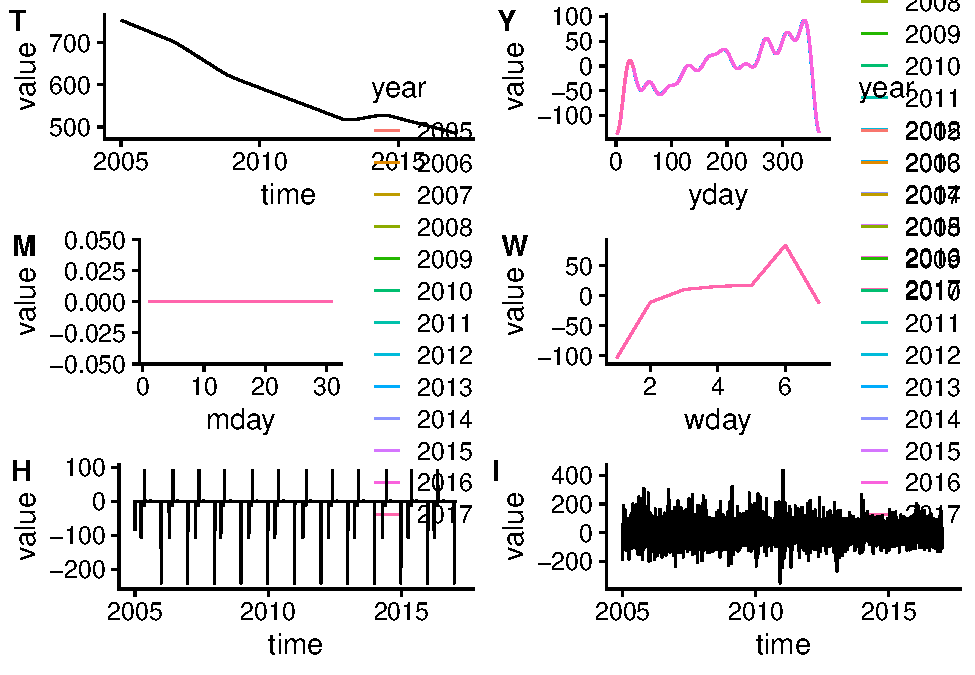
\includegraphics[width=1\linewidth]{overview_files/figure-latex/unnamed-chunk-6-1} \end{Schunk}

\hypertarget{casualties-stl}{%
\paragraph{Casualties, STL}\label{casualties-stl}}

\begin{Schunk}
\begin{Soutput}
#> Warning: Removed 35 row(s) containing missing values (geom_path).
\end{Soutput}

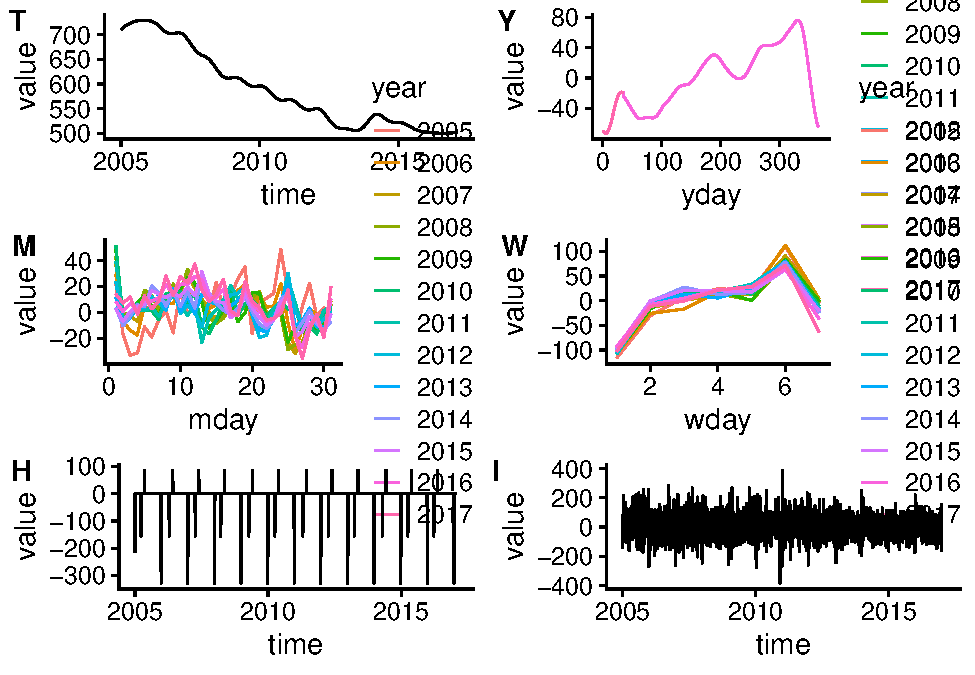
\includegraphics[width=1\linewidth]{overview_files/figure-latex/unnamed-chunk-7-1} \end{Schunk}

\hypertarget{oos-forecast-plots}{%
\subsubsection{OOS Forecast plots}\label{oos-forecast-plots}}

\hypertarget{casualties-prophet-1}{%
\paragraph{Casualties, Prophet}\label{casualties-prophet-1}}

\begin{Schunk}

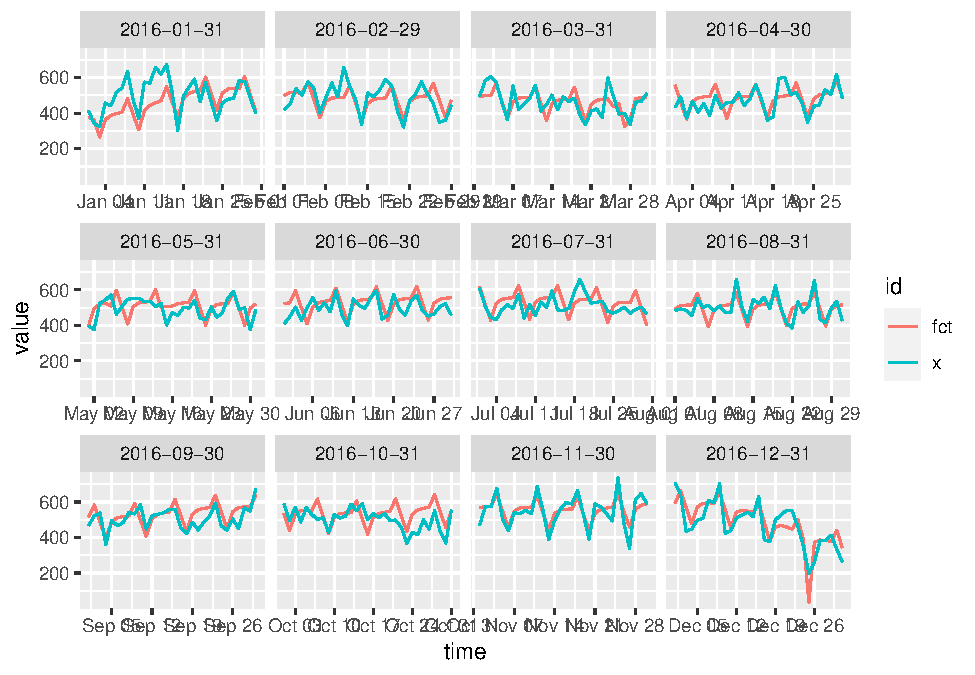
\includegraphics[width=1\linewidth]{overview_files/figure-latex/unnamed-chunk-8-1} \end{Schunk}

\hypertarget{casualties-dsa-1}{%
\paragraph{Casualties, DSA}\label{casualties-dsa-1}}

\begin{Schunk}

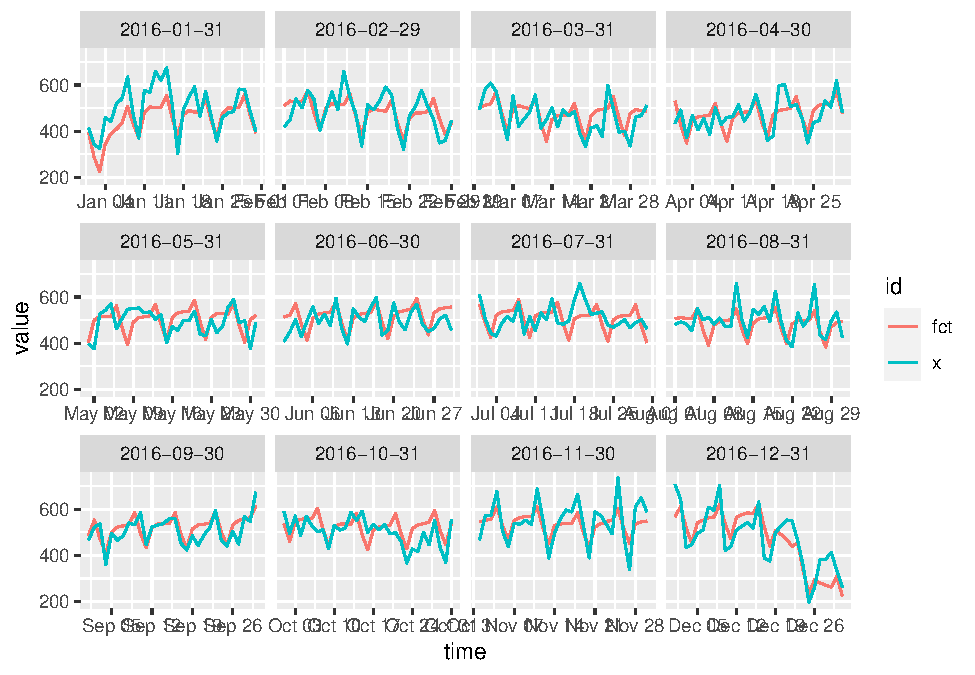
\includegraphics[width=1\linewidth]{overview_files/figure-latex/unnamed-chunk-9-1} \end{Schunk}

\hypertarget{casualties-stl-1}{%
\paragraph{Casualties, STL}\label{casualties-stl-1}}

\begin{Schunk}

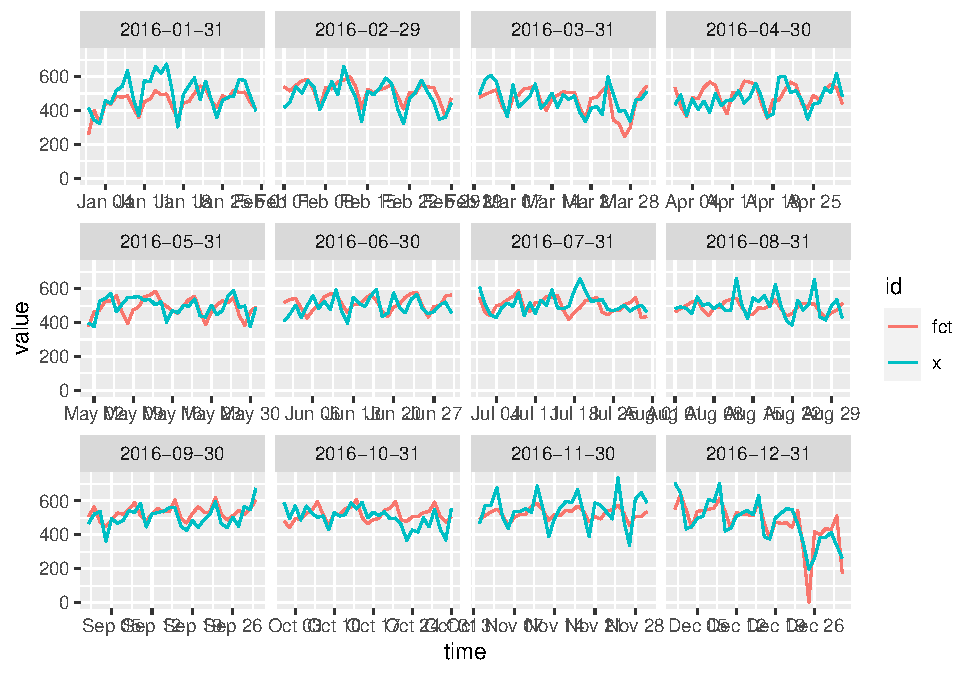
\includegraphics[width=1\linewidth]{overview_files/figure-latex/unnamed-chunk-10-1} \end{Schunk}

\bibliography{overview.bib}

\address{%
Christoph Sax\\
University of Base\\%
line 1\\ line 2\\
%
\url{https://journal.r-project.org}%
\\\textit{ORCiD: \href{https://orcid.org/0000-0002-9079-593X}{0000-0002-9079-593X}}%
\\\href{mailto:author1@work}{\nolinkurl{author1@work}}
}

\address{%
Author Two\\
Affiliation 1\\%
line 1 affiliation 1\\ line 2 affiliation 1\\
Affiliation 2\\%
line 1 affiliation 2\\ line 2 affiliation 2\\
%
\url{https://journal.r-project.org}%
\\\textit{ORCiD: \href{https://orcid.org/0000-0002-9079-593X}{0000-0002-9079-593X}}%
\\\href{mailto:author2@work}{\nolinkurl{author2@work}}
}

\address{%
Author Three\\
Affiliation\\%
line 1 affiliation\\ line 2 affiliation\\
%
\url{https://journal.r-project.org}%
%
\\\href{mailto:author3@work}{\nolinkurl{author3@work}}
}

